\subsection{Tradeoffs of Group Testing}
\lecture{13 May}

As a final remark to group testing, let us consider the tradeoffs between the five dimensions of group testing:
\begin{enumerate}
    \item Non-adaptive / adaptive: The group testing is done a single round for non-adaptive ones. For adaptive ones it can be done with multiple round, and future rounds can utilize the knowledge gained from past rounds.
    \item The number of tests $m$: we often want $m=O(k\log n)$ since it is the information-theoretic bound. In reality, it might be hard to reach.
    \item Noisy / noiseless: whether you can trust the test results.
    \item Decode complexity: we want it to be $O(k\log n)$, $O(k\,\mathrm{polylog}\,n)$, or $\mathrm{poly}(k\log n)$.
    \item Number of false positives and false negative (\#FP \& FN): should be $O(1)$ or $o(k)$.
\end{enumerate}
Our preferred combination would be to have a nonadaptive noiseless group testing with $O(k\log n)$ tests, $O(k\,\mathrm{polylog}\,n)$ decoding complexity, and 0 FN \& FP with high probability.

The current state of the art can only achieve any combination of four of the above, but never all five.
\begin{enumerate}
    \item If we give up the first: then we can use the adaptive binary search method as introduced in the start of \autoref{sec:w12_bin_GT}.
    
    \item If we give up the second: in GROTESQUE \cite{grotesque_GT} and SAFFRON \cite{saffron_GT}, we have the number of tests being $m=O(k\log k\log n)$.
    
    \item If we give up the third: consider the binary tree folding as introduced in \autoref{sec:w12_bin_GT}. Normally when the tests are noiseless, we can cut all the leaves to a node if it is tested to be negative. However, for the case where the tests are noisy, say $\mathrm{BSC}(p)$-noisy, then we must do more tests to be sure. Setting a threshold for the amount the negative results that we accept it as truly being negative, the complexity becomes $p^{c\log k}$.
    
    \item If we give up the fourth: we can relax the decoding complexity to $mn$ by using a random testing matrix $A$ with $\mathrm{Ber}(1/ck)$ entries. Every $y_i=\min(Ax,1)$ should hence behave like $\mathrm{Ber}(1/2)$ so that we can actually learn something from $y_i$ (the maximum entropy Bernoulli random variable). To decode, one computes $d_\mathrm{H}(y,Ax_i)$ for all $i\in[n]$. If the value is \textit{low}, then the $i$th person is sick; if the $i$th person is healthy, the Hamming distance should be $m/2$. Hence, we can set the threshold at about $m/3$. This is the COMP algorithm proposed by Chan et al. \cite{COMP_GT}. If done in a brute force manner, the decoding complexity is $m\binom{n}{k}$. Note that in real world applications: in the case of disease control, $n$ is often of the order of hundreds; in communication, $n$ is often of the order of $30^{160}$.

    \item If we give up the fifth: the number of FN and FP is of order $\varepsilon k$.    
\end{enumerate}
Let us discuss a bit more when we give up the fifth criterion and enforce the first four criteria. The current bound is
\begin{equation}
    \#\mathrm{FP \& FN} = O\left(2^{-\sqrt{\lg n}}k\right)
\end{equation}
on average.

In GROTESQUE \cite{grotesque_GT} and SAFFRON \cite{saffron_GT}, they consider the following scheme for group testing:
\begin{figure}[H]
    \centering
    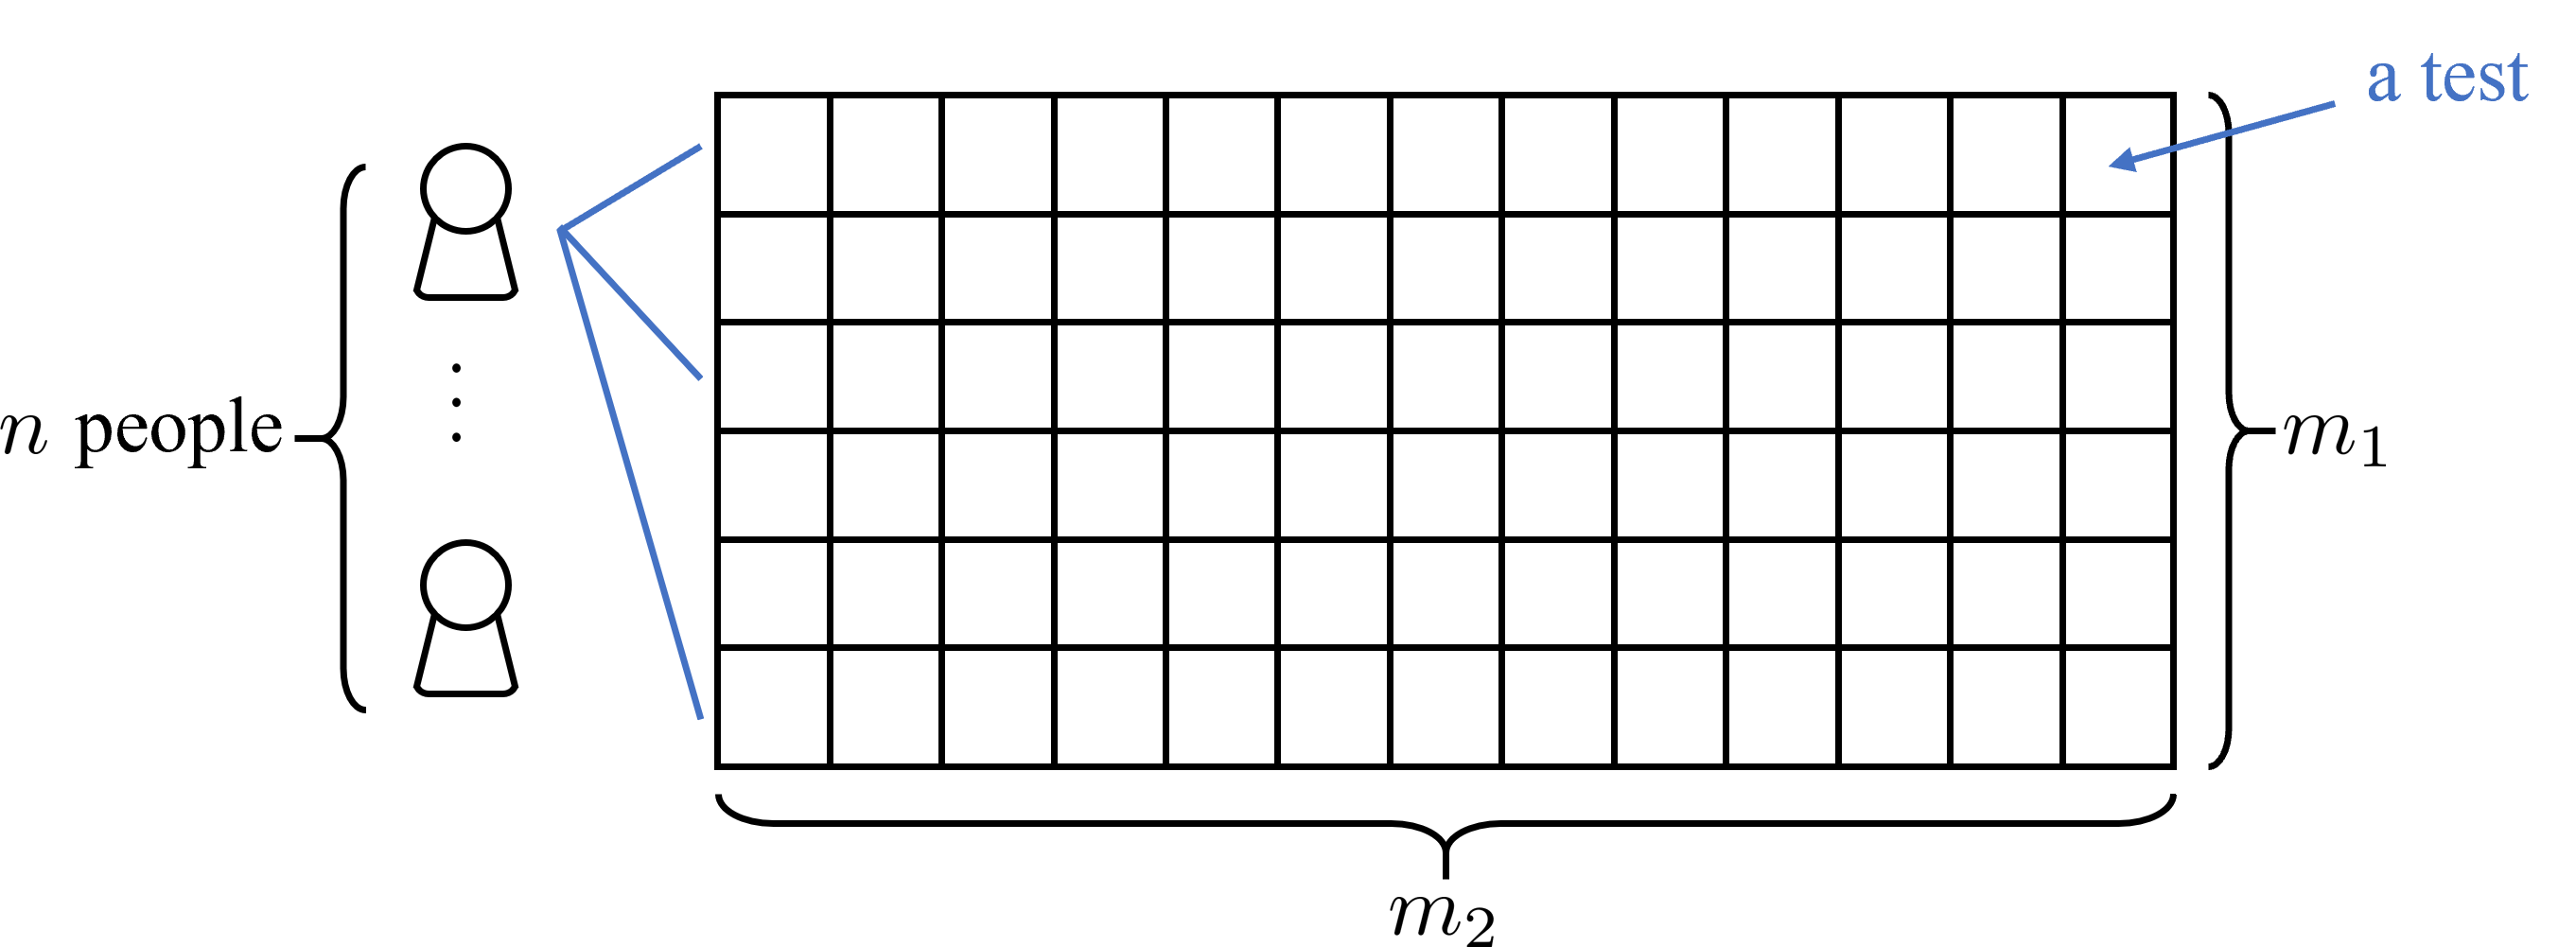
\includegraphics[width=0.8\linewidth]{figures/w13_GT_setup.png}
    \caption{A general setup for group testing}
    \label{fig:w13_GT_setup}
\end{figure}
See \autoref{fig:w13_GT_setup}, there are a total of $n$ people, each with an ID number of length $m_2$. Each person chooses three rows (out of the total $m_1$ rows) and fill in their ID number. Tests will be conducted for all the $m = m_1 \cdot m_2$ boxes, and the corresponding numbers in each boxes will show up if at least one person choosing the box is sick. For starters, let us choose an ID string of length $m_2$, with $m_2 = 100\lg n$ and $m_1=100k$.

Assume that we can always recover the person of an ID string if that string is the only one occupying a row. What happens when multiple people choose the same row? The simplest scheme is to simply give up on any overlaps. Out of the $100k$ rows, there should be $3k$ rows that are sick, so the occupancy rate of sick rows is $3\%$. In other words, any random person has a probability of $(3\%)^3$ to pick exactly three sick rows. So the number of FPs and FNs is $(3\%)^3k = \varepsilon k$.

How do we fix this? The following discussion follows from the work by Guruswami and Wang \cite{exponent_optimal_GT}.

This time, let us set the length of the ID strings to $\lg n$, with $m_2 = 100\sqrt{\lg n}$ and $m_1=100k\sqrt{\lg n}$. The amount of tests doesn't change, as it is still of the order $O(k\lg n)$. Further, each person picks $10$ rows to fill in their ID a total of $10$ times (if a row ends without completing the ID string, the string continues on another row). In this setup, the occupancy rate of sick rows is
\begin{equation*}
    \frac{10\sqrt{\lg n} \times k}{100 k \sqrt{\lg n}} = 10\%.
\end{equation*}
A na\"ive analysis of the number of FPs and FNs will be
\begin{equation*}
    \mathrm{Pr}\{\text{all rows chosen are occupied}\} = \left(10\%\right)^{10\sqrt{\lg n}}.
\end{equation*}
Hurray! This is no longer a constant, but a decreasing function of $n$. However, the above analysis is crude, since one cannot identify themselves by using a single row. Instead, we should use Hoeffding's inequality:
\begin{align}
    \mathrm{Pr}\{\text{have fewer than }\sqrt{\lg n}\text{ rows left}\} &< \exp\left(-\text{const.}\times\text{deviation}\right) \\
    &= \exp\left(-c\cdot 8 \sqrt{\lg n}\right).
\end{align}
On average, one should only loose $1$ row due to it being occupied, the worst case is loosing $9$ rows, hence the deviation is $8$ rows. Finally, we have
\begin{equation}
    \#\text{FP\&FN} = O\left(2^{-\sqrt{\lg n}}k\right) = o(k).
\end{equation}
We have achieved our goal.

Some final remarks on how one decode themselves: 
\begin{remark}
    One can apply Reed--Solomon code to the $10\sqrt{\lg n}$ rows a person chooses to ensure any $\sqrt{\lg n}$ rows given can be used to decode the corresponding string.

    Furthermore, how do we know whether two different rows correspond to the same person? The solution is simple, we simply add hash, say of length $50\sqrt{\log n}$, to the front of each row. This was also proposed in the work by Guruswami and Wang \cite{exponent_optimal_GT}.
\end{remark}

\begin{remark}
    Instead of having $(\lg n)^{1/2}$, other exponents can be used.

    Say each string of ID is of length $(\lg n)^{2/3}$, each person chooses enough rows such that $10$ copies of the ID are written. Let $m_1 = 100k(\lg n)^{2/3}$, $m_2 = 100(\lg n)^{1/3}$, and the length of hash is $50(\lg n)^{1/3}$. What happens now? The probability of having the chosen rows being too occupied will now be $\exp(-c\cdot 8(\lg n)^{2/3})$, this is much better than before! However, hash collisions may occur. The probability of hash collision will be $2^{-(\lg n)^{1/3}}$. The final rate of FPs and FNs will be the max of the two.

    But wait, we can apply the same scheme again! We add hash values to the previous hash values that have collision. Then the number of FPs and FNs will be
    \begin{equation*}
        2^{-(\lg n)^{2/3}}k.
    \end{equation*}
    Why stop here? Applying this scheme again, we will have $2^{-(\lg n)^{3/4}}k$. Eventually, we can achieve
    \begin{equation}
        2^{-(\lg n)^{1-1/\tau}} k.
    \end{equation}
\end{remark}















%%%%%%%%%%%%%%%%%%%%%%%%%%%%%%%%%%%%%%%%%%%%%%%%%%%%%%%%%%%%

\section{Distributed Matrix Multiplication} \label{sec:w13_distr_mat_mult}
Consider given the task of calculating the matrix product
\begin{equation*}
    \left[\begin{matrix}
        A_{11} & A_{12} \\
        A_{21} & A_{22}
    \end{matrix}\right] \left[\begin{matrix}
        B_{11} & B_{12} \\
        B_{21} & B_{22}
    \end{matrix}\right] = \left[\begin{matrix}
        A_{11}\cdot B_{11} + A_{12}\cdot B_{21} & A_{11}\cdot B_{12} + A_{12}\cdot B_{22} \cdot \\
        A_{21}\cdot B_{11} + A_{22}\cdot B_{21} & A_{21}\cdot B_{12} + A_{22}\cdot B_{22}
    \end{matrix}\right],
\end{equation*}
it requires $8$ scalar multiplications. If we distribute this $8$ tasks to $8$ GPUs to compute and output the result only after all $8$ GPUs finish, our computation will be vulnerable when some GPUs are slow. This may be due to some randomness, overheating, power outage, or our favorite, Microsoft system auto-update.

We can partition $A$ into
\begin{equation*}
    A = \left[\begin{matrix}
        A_1 \\ A_2
    \end{matrix}\right] \Rightarrow \tilde{A}_{2/3} \defeq \left[\begin{matrix}
        A_1 \\ A_2 \\ A_1 + A_2
    \end{matrix}\right].
\end{equation*}
If we compute the product $\tilde{A}B$, and distribute the task $A_1B$, $A_2B$, and $(A_1+A_2)B$ to three separate processors, we can recover $AB$ once any two finish. Since matrix addition is really cheap ($O(n)$) in comparison to multiplication ($O(n^3)$). We only care about reducing the multiplication count.

Let us continue on with this strategy, and define
\begin{equation*}
    A = \left[\begin{matrix}
        A_1 \\ A_2 \\ A_3
    \end{matrix}\right] \Rightarrow \tilde{A}_{3/5} = \left[\begin{matrix}
        A_1 \\ A_2 \\ A_3 \\ A_1+A_2+A_3 \\ A_1+2A_2+3A_3
    \end{matrix}\right],
\end{equation*}
this is a 3-out-of-5 system (3/5-system). By incorporating more redundant tasks, we can prevent our computation being affected by slow GPUs. In fact, by employing an $[n,k]$-Reed--Solomon code, we can implement a $k/n$-system. This is called the \textit{polynomial code}, and will be discussed later in \autoref{sec:w16_polynomial_code}.

We can do better! Besides defining $\tilde{A}_{2/3}$, we also define $\tilde{B}_{2/3} = [B_1,B_2,B_1+B_2]$. Then we can use $9$ GPUs to compute $\tilde{A}_{2/3}\tilde{B}_{2/3}$, and requiring only $5$ of them to obtain $AB$. Its extension will be a two-dimensional Reed--Solomon code.

In general, we find good matrices $G$ and $H$ as row and column operations, respectively, and compute
\begin{equation}
    \tilde{A}\tilde{B} = (GA)(BH).
\end{equation}

\subsection{Polynomial Codes} \label{sec:w13_polynomial_codes}
Let us introduce the method of polynomial codes \cite{polynomialcodes}: For $A$ and $B$ being $n\times n$ matrices, consider computing
\begin{equation}
    (\vec{g}_s\cdot A)(B\cdot \vec{h}_s)
\end{equation}
at the $s$th GPU, with vectors
\begin{equation}
    \vec{g}_s = \left[\begin{matrix}
        1 & \xi_s & \cdots & \xi_s^{n-1}
    \end{matrix}\right], \vec{h}_s = \left[\begin{matrix}
        1 \\ \xi_s^n \\ \vdots \\ \xi_s^{n^2-n}
    \end{matrix}\right],
\end{equation}
and $\xi_1$, $\ldots$, $\xi_s$, $\ldots$ are all distinct.

\begin{theorem}[Polynomial Codes]
    Any $n^2$ GPUs recovers $AB$.
\end{theorem}
\begin{proof}
    Observe that
    \begin{equation*}
        \vec{g}_s\cdot AB\cdot \vec{h}_s = \trace{\vec{h}_s\vec{g}_s\cdot AB} = \langle \vec{h}_s\vec{g}_s,AB\rangle,
    \end{equation*}
    where $\langle\cdot,\cdot\rangle$ is the Frobenius inner product. Since $\vec{h}_s\vec{g}_s$ forms a matrix basis $X_s$: we can compute $n^2$ of
    \begin{equation*}
        \langle X_1,AB\rangle = \trace{X_1(AB)}, \langle X_2,AB\rangle = \trace{X_2(AB)}, \ldots
    \end{equation*}
    so as to finally obtain $AB$.
\end{proof}

\subsection{MatDot}
Let us introduce the method of MatDot \cite{MatDot}\footnote{To be frank, I think the polynomial codes is more related to ``dot'' product.}: Let the $s$th CPU compute the product
\begin{equation}
    A\vec{x}_s\vec{y}_sB,
\end{equation}
with $\vec{x}_s = [1,\xi_s,\ldots,\xi_s^{n-1}]^\transpose$ and $\vec{y}_s = [\xi_s^{n-1},\ldots,\xi_s,1]$. Again, all the $\xi_s$'s are distinct.

\begin{theorem}[MatDot]
    Any $(2n-1)$-subset of $A\vec{x}_s\vec{y}_sB$ recovers $AB$.
\end{theorem}
\begin{proof}
    Observe that
    \begin{equation*}
        \vec{x}_s\vec{y}_s = \left[\begin{matrix}
            \xi_s^{n-1} & \cdots & \xi_s & 1 \\
            \vdots & \ddots & & \xi_s \\
            \xi_s^{2n-3} & & \ddots & \vdots \\
            \xi_s^{2n-2} & \xi_s^{2n-3} & \cdots & \xi_s^{n-1}
        \end{matrix}\right]
    \end{equation*}
    is a Toeplitz matrix. And any $(2n-1)$-subset of $A\vec{x}_s\vec{y}_sB$ spans all Toeplitz matrix, which includes the identity matrix $\mathbbm{1}$. Henceforth, we can obtain $A\mathbbm{1}B=AB$ from linear combinations of $2n-1$ $A\vec{x}_s\vec{y}_sB$'s.
\end{proof}

\subsection{Strassen's Method}
The classical method for fast $2\times2$ matrix multiplication is the Strassen method, requiring only $7$ scalar multiplications. See the terms below
\begin{align*}
    S^{(1)} &= (A_{11} + A_{22}) (B_{11} + B_{22}), \\
    S^{(2)} &= (A_{21} + A_{22}) B_{11}, \\
    S^{(3)} &= A_{11} (B_{12} - B_{22}), \\
    S^{(4)} &= A_{22} (-B_{11} + B_{21}), \\
    S^{(5)} &= (A_{11} + A_{12}) B_{22}, \\
    S^{(6)} &= (-A_{21} + A_{11}) (B_{11} + B_{12}), \\
    S^{(7)} &= (A_{12} - A_{22}) (B_{21} + B_{22}).
\end{align*}
Let $C=AB$, then
\begin{align*}
    C_{11} &= S^{(1)} + S^{(4)} - S^{(5)} + S^{(7)}, \\
    C_{12} &= S^{(3)} + S^{(5)}, \\
    C_{21} &= S^{(2)} + S^{(4)}, \\
    C_{22} &= S^{(1)} - S^{(2)} + S^{(3)} + S^{(6)}.
\end{align*}

If we want to extend Strassen's method to distributed computing, we should add some redundancy: consider
\begin{align*}
    S^{(8)} &= (A_{11} + 2 A_{21}) (-B_{11} + B_{12}), \\
    S^{(9)} &= (A_{12} + 2 A_{22}) (-B_{21} + B_{22}).
\end{align*}

\begin{theorem}
    Any $8$ of $S^{(i)}$'s recover $C=AB$.
\end{theorem}
\begin{proof}
    Consider the product:
    \begin{equation*}
        \text{linear combination of $C_{ij}$'s} = \left[\begin{matrix}
            1 & 2
        \end{matrix}\right] C \left[\begin{matrix}
            -1 \\ 1
        \end{matrix}\right] = S^{(8)} + S^{(9)} = \text{linear combination of $S^{(1)}$ to $S^{(7)}$},
    \end{equation*}
    where the last equality is by knowing that the Strassen's method works. The linear combination is
    \begin{equation}
        (1,-4,3,-3,2,2,-1)\cdot(S^{(1)},\ldots,S^{(7)}) = S^{(8)} + S^{(9)}.
    \end{equation}
    Henceforth, if any single one of the $S^{(i)}$'s is missing, we can use the above linear equation to recover it.

    If we want to counter $2$ missing data, we can construct
    \begin{equation*}
        \left[\begin{matrix}
            3 & -1
        \end{matrix}\right] C \left[\begin{matrix}
            1 \\ 2
        \end{matrix}\right] = S^{(10)} + S^{(11)}.
    \end{equation*}
    Then we just need to solve
    \begin{equation}
        \left[\begin{array}{ccccccc:cccc}
            1 & -4 & 3 & -3 & 2 & 2 & -1 & -1 & -1 & 0 & 0 \\
            1 & 1 & 4 & 2 & 3 & -2 & 3 & 0 & 0 & -1 & -1
        \end{array}\right] \left[\begin{array}{c}
            S^{(1)} \\ \vdots \\ S^{(7)} \\ \hdashline S^{(8)} \\ \vdots \\ S^{(11)}
        \end{array}\right] = 0 \label{eq:w13_distributed_Strassen}
    \end{equation}
    to recover the missing terms. This is possible due to the fact that any $2\times 2$ minor (containing at least one column from the first 7 columns) of the matrix on the left in \autoref{eq:w13_distributed_Strassen} is invertible.
\end{proof}
This set of combinations is found by brute force via a computer.




\begin{remark}
    It should be noted that Strassen's method is not optimal, as faster methods exist, such as the Coppersmith-Winograd method.
\end{remark}

\begin{remark}
    Interestingly enough, just a few days after the lecture, the team of Google Deepmind published a result on fast matrix multiplication from their AI AlphaTensor on 15th of May, 2025. The traditional method of multiplying a $4\times4$ matrix using the Strassen's method requires $49$ scalar multiplications. Amazingly, the method proposed by Deepmind requires only $48$ scalar multiplications! What a breakthrough.
\end{remark}

\subsection{Laderman's Method}
The Laderman's method \cite{Laderman3x3} deals with fast $3\times 3$ matrix multiplication, requiring only $23$ scalar multiplications! I will not explicitly write out the $23$ terms $L^{(1)}$ to $L^{(23)}$, however, we will discuss an extension of it to the distributed case.

Compared to the direct method requiring $3^3=27$ multiplications, we can add $3$ more redundancies and still outperform direct computation. We can obtain $L^{(24)}$, $L^{(25)}$ and $L^{(26)}$ from the product
\begin{equation}
    \left[\begin{matrix}
        2 & 1 & 3
    \end{matrix}\right] C \left[\begin{matrix}
        2 \\ -1 \\ 3
    \end{matrix}\right] = L^{(24)} + L^{(25)} + L^{(26)},
\end{equation}
just like what we did for the distributed case of Strassen's method.

